We have presented a method of nonlinear dimensionality reduction that is compatible with the scale and composition of modern biobanks. With UMAP and HDBSCAN($\hat{\epsilon}$) we have uncovered a wide variety of patterns of fine-scale population structure in every biobank studied. Since the publication of \hyperref[chap:chapter2]{Chapter~2} , UMAP has become a standard method for visualization and exploratory data analysis in population genetics. Given the demand for cluster extraction noted in \hyperref[chap:chapter3]{Chapters~3} and \hyperref[chap:chapter4]{4}, it is possible that HDBSCAN($\hat{\epsilon}$)---or some other density clustering method---could see similar adoption.

The timing of UMAP coincides fortuitously with the growth of biobanks and the genomic revolution. Writing in his review of TDA in 2018, Wasserman asked, ``is it possible to derive low dimensional embedding methods that explicitly preserve topological features of the data? This is an interesting open question.''\citep{wasserman_topological_2018} This review was published in the same year that UMAP, an explicitly topological method, was released. Topological analysis and density clustering seem especially well-suited to the task of understanding population structure in diverse biobanks.

\section{The value of visualization}

In \hyperref[chap:chapter3]{Chapter~3} we describe the relationship between dimensionality reduction and biological data as analogous to that of microscopes and biological samples. This analogy has been made before with respect to mathematics in general\citep{cohen_mathematics_2004}. Though analyses, inferences, and models can shed light on the biological world, there is an inherent value to being able to literally see your data and understand its structure. Among the most cited papers in population genetics is ``Genes mirror geography within Europe''\citep{novembre2008europe}---although isolation-by-distance had been characterized almost a century earlier, the figure of the top principal components superimposed over Europe was an elegant illustration of the geographical distribution of human genetic variation.

With UMAP, we are able to map complex genetic structure down to $2$ or $3$ dimensions for visualization, examine the fine-scale structure that a method like PCA compresses, while preserving interesting signal in the data. Using auxiliary data---geographic data, population labels, phenotypic information, environmental variables, etc.---we can visually scan for patterns and generate hypotheses. In \hyperref[chap:chapter2]{Chapter~2} we present a variety of visualization methods, including colouring points by admixture levels to uncover gradients in ancestry and converting 3D UMAP coordinates to RGB colour levels for colouring maps. One common method used in single-cell studies is to colour UMAP plots by gene expression levels (e.g. \citep{jessa_stalled_2019} Figure~4h). A similar approach could be used in exploring allele distributions by clusters to see whether they are relatively more common in different populations---one such method, called the Allele Dispersion Score, was proposed by Correard et al. in 2022\citep{correard_allele_2022}. Though UMAP figures are now standard in genetic studies, most are limited to a simple 2D scatterplot coloured by some population label---in every biobank, there is certainly value in exploring deeper and using other variables.

There is also value in going beyond static $2$D figures. Software libraries such as plotly\citep{plotly} can generate interactive figures, are available for Python and R, and are straightforward to implement. Interactive exploration can assess how individual points fit within larger projections, rapidly identifying patterns or using them for diagnostics. Working in $3$D is much easier when the figures are interactive, and we have, e.g., explored the relationships between individuals and populations in the UKB. Finally, as noted in \hyperref[chap:chapter4]{Chapter~4}, clustering works well in dimensions above $2$---while it can be tempting to delineate clusters from $2$D figures alone, the jump from $3$ to $2$ dimensions can lose information about how points are related to one another. There is value in using information from higher dimensions to aid visualization in lower dimensions and, despite UMAP's now-widespread use, its ability to work in $3$ or more dimensions is, in the view of the author, underappreciated.

\section{Implications for biomedical and epidemiological research}

Biobanks are as complex as they are rich. Across visualizations in \hyperref[chap:chapter2]{Chapters~2} and \hyperref[chap:chapter4]{4}, we see patterns. Some appear quickly at the population level, as in Figure~\ref{fig:fig6} where we see population-level differences in height and blood cell count; others require iterative smoothing, such as  Figure~\ref{fig:smoothed_phenos} where we see residual structure in phenotypes after removing the effects of the top $40$ PCs. These patterns also appear in behavioural measures, such as smoking in Figure~\ref{fig:supp_ukb_smoking}. Figures~\ref{fig:supp_montage_ukbb_ns} and \ref{fig:supp_montage_ukbb_ew} show how geographic structure is closely tied to genetic structure. Using variables like admixture proportions, country of birth, immigration history, environmental data, etc, we see the difficulty of disentangling genetic and environmental effects becomes evident.

These many overlapping patterns  undercut the idea that a relationship between genetics and phenotype or disease state implies an underlying genetic architecture. Consider a thought experiment\citep{rose_sick_2001}: if there were a genetic population in which everyone is a smoker, we would erroneously conclude that lung cancer is a genetic disease because of a deep entanglement between environment and genetics. 

-could have a pgh here about type genomes
-label-agnostic
-labels shape how we perceive populations and also guide how we build them (e.g. we want to match methods to labels)

-should take an approach the benefits everyone, ML methods can perpetuate bias because they seem ``objective''\citep{gebru_race_2020}

Density clustering with UMAP has potential application for defining study populations. It has several advantages over methods based on, e.g., $K$-means clustering: it clusters all or almost all individuals, even those with recent admixture or from uncommon ancestries; it is does not assume a number of populations $K$; it does not require reference panels; its assumptions of the structure of genetic data are more realistic. It also has advantages over variables like self-identification or country of birth that, though sometimes used as proxies for population structure, are not actually genetic information--- even then, we see in \hyperref[chap:chapter4]{Chapter 4} that there is differential response in identification with, e.g., many individuals from non-majority populations simply identifying as ``other''.

 Approximately $86\%$ of genomic studies by 2021 were based on individuals of European ancestry, an increase from $81\%$ in 2016\citep{fatumo_roadmap_2022,kaplan_polygenic_2022}. Many studies have data from non-European individuals (there are thousands within the UKB, for example) but discard data citing concerns around low sample sizes or issues with population structure\citep{ben-eghan_dont_2020}. In principle, an approach using UMAP and HDBSCAN($\hat{\epsilon}$) could alleviate some of these problems: first, by defining study populations, and second, by revealing fine-scale population structure and its many correlates. This has several advantages over methods based on, e.g. $K$-means clustering: it clusters all or almost all individuals, even those with, e.g., recent admixture; it is does not require assumptions about $K$; it does not require reference panels; its assumptions of the structure of genetic data are more realistic. It also has advantages over variables like self-identification or country of birth that, though sometimes used as proxies for population structure, are not actually genetic information--- even then, we see in \hyperref[chap:chapter4]{Chapter 4} that there is differential response in identification with, e.g., many individuals from non-majority populations simply identifying as ``other''.

\begin{figure}[ht]
\centering
\begin{subfigure}{0.45\linewidth}
    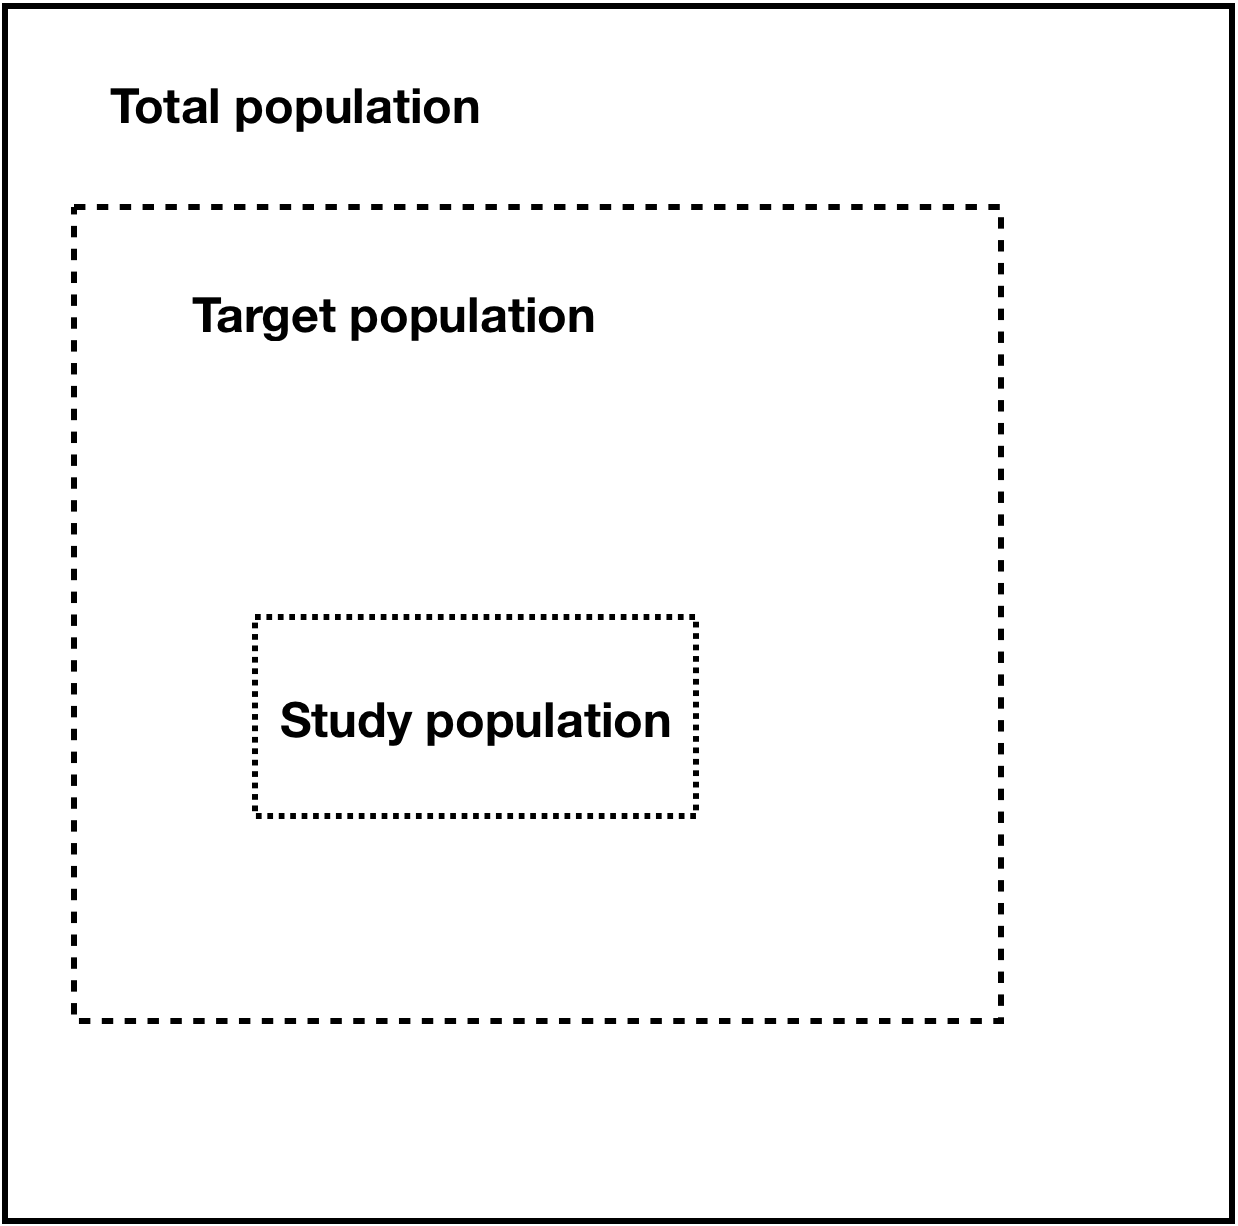
\includegraphics[width=\linewidth]{main_figures/discussion/populations_1.png}
    \caption{}
    \label{fig:statistical_populations1}
\end{subfigure}
\hfill
\begin{subfigure}{0.45\linewidth}
    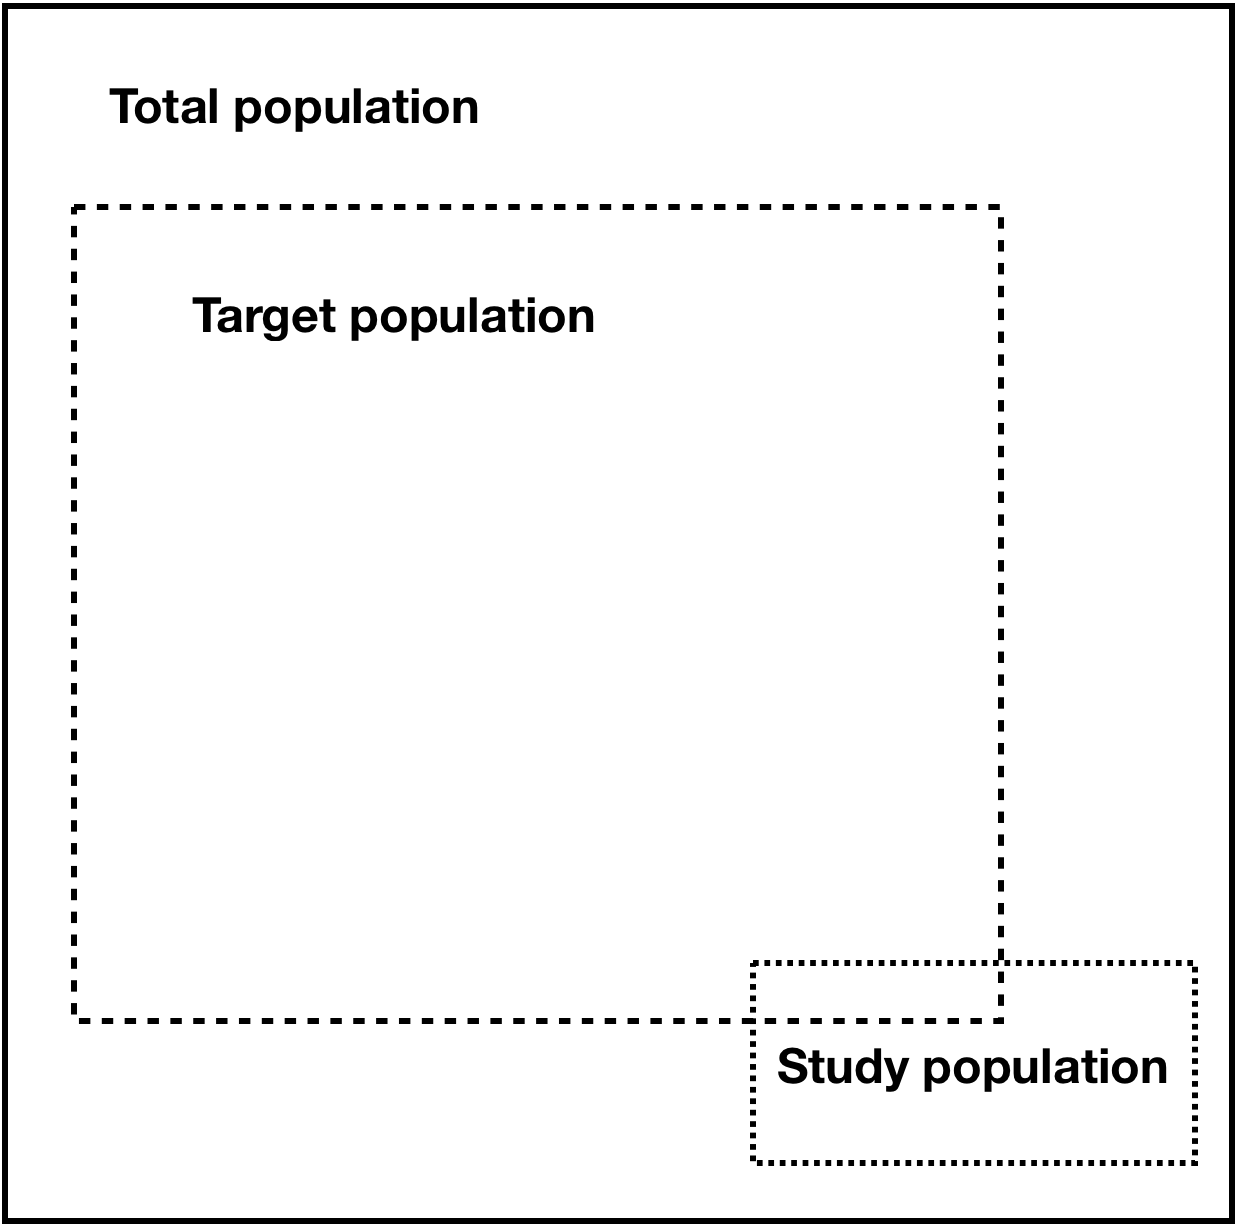
\includegraphics[width=\linewidth]{main_figures/discussion/populations_2.png}
    \caption{}
    \label{fig:statistical_populations2}
\end{subfigure}
\caption[The relationship between target and study populations]{\textbf{The study population should match the target population.} In \textbf{(a)}, the study population is a subset of the target population, so inferences drawn from it will apply to the target population. In \textbf{(b)}, the study population is not fully a subset of the target population, so its inferences will be less reliable.}
\label{fig:statistical_populations}
\end{figure}

In inferential statistics, we require some definitions of ``population'', shown in Figure~\ref{fig:statistical_populations} . To establish the scope of study we define a target population (the group to whom the research applies) and the study population (the group which is covered by the study and is, ideally, drawn from the target population)\citep{statcan2003}. Biobanks are generally not random samples of a population and suffer from selection bias\citep{huang_representativeness_2021}; there are genetic biases in enrolment itself\citep{pirastu_genetic_2021,benonisdottir_studying_2023}. The target population for a study may be, e.g., all European-ancestry individuals---but if there is significant bias in the composition of a biobank, the study population is not aligned with the target population and the inference may not be reliable. As such, though we have a methodology to define populations, any analyses are necessarily conditioned on the data sources themselves.

\section{Clustering in population genetics}
% we could just draw... but we want something principled too
Unlike problems like classification, clustering does not have a well-defined ground truth, and even the most basic definition, such as ``similar points are grouped together and dissimilar points are grouped separately'', can be self-contradictory\citep{ben-david_clustering_2018}. In a genetic cluster from \hyperref[chap:chapter4]{Chapter~4}, individuals in may be closely related to their immediate neighbours, but not to those in a far end of a cluster; they are grouped by similarity in one sense, but not separated by dissimilarity. Different inputs, algorithms, and parametrizations will yield different results. Though various quality metrics exist, even untrained humans excel at assessing arbitrary $2$D clustering\citep{lewis_human_2012}---there is an element of ``I know it when I see it''. Paired with auxiliary data, e.g. country of birth, we can explore population structure much more effectively than before.

\begin{figure}[h]
\centering
    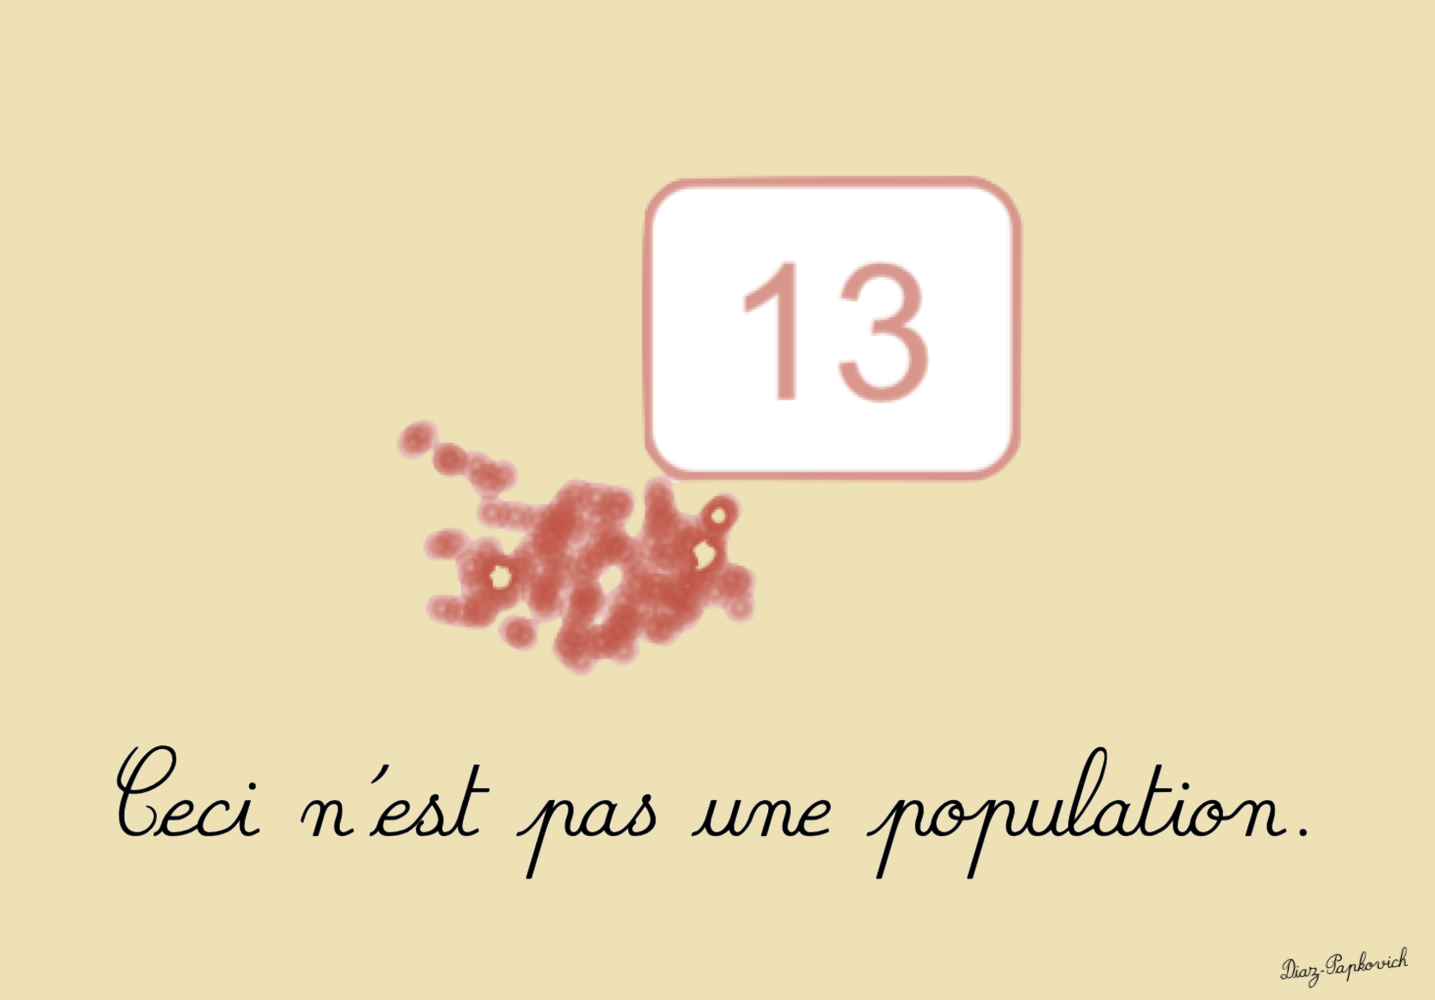
\includegraphics[width=0.75\linewidth]{main_figures/discussion/magritte.png}
\caption[The treachery of clustering]{\textbf{A cluster is only an abstraction, albeit a useful one.}}
\label{fig:magritte}
\end{figure}

Clusters are a discrete encapsulation of genetic ancestry, which is a continuous and multidimensional variable. Clusters that are clearly separated in one sample will ultimately fall into a continuum among larger and more diverse samples\citep{lewis_getting_2022}. We have seen through this thesis that clusters can split, merge, reappear, or disappear, in the same vein that objects may appear or disappear in microscopy depending on the depth and focus and type of microscope used. It would be folly to look at, e.g., a $2$D slice of a single cell and its sub-cellular components at one single time point and to conclude that this image defines the ``real'' cell. It is, however, a useful representation of the structure of the cell---provided we keep in mind that everything we see is conditioned on the sample (e.g. the cell type and state, the health of the organism, the environment in which the cell is viewed, etc).

These same conditions apply to data. Data sets do not spring forth naturally; they are sampled, collected, processed, and are products of societies and institutions situated within their own contexts and biases\citep{dignazio_data_2020}. Population labels are an excellent example, since we often use them as shorthand for clusters and populations. In the UKB, there are $20$ unique values for ``ethnic background'' (see Table~\ref{table:ukb_eb_options}) and they are selected in a nested manner (first you select from a list of ``ethnic groups'', then from a second list of ``ethnic backgrounds''). It is not possible to identify as, for example, ``Chinese British'' or ``Mixed Black and Asian'', though there are certainly individuals who would select those labels. In British English, ``Asian'' typically refers to individuals with South Asian ancestry, while in American English, it refers to East Asian. These details shape not only our perceptions of our own work, but also the perceptions of those who consume our research. When we work with clusters and we use labels, we are drawing maps of an unknown territory.

It is erroneous to describe clusters as ``objective'' measures of human population structure, both for the aforementioned reasons, and also because clustering changes based on many subjective inputs: algorithms, hyperparameters, subsets of data, etc\citep{watson_philosophy_2023}. The cost of epistemological ignorance here varies, but at its most extreme, it can lead to misinterpretation and misuse in scientific racism\citep{panofsky_genetic_2019,panofsky_how_2021}. Like any powerful tools, we must understand the strengths and limitations of dimensionality reduction and clustering in population genetics and use them responsibly, particularly for visualizations\citep{carlson_counter_2022}.

Still, as we have seen throughout this work (particularly \hyperref[chap:chapter4]{Chapter~4}), clusters are useful abstractions. The structure they find is ``real'' in the sense that it is a discrete measure of relatedness between individuals, with the caveat that it the structure identified is conditioned on the data and methods. When we require a genetic definition of a population, such as to calculate a MAF or train/test a PGS or to explore biobank data efficiently, the approach of using UMAP and HDBSCAN($\hat{\epsilon}$) shows great promise.

\section{Limitations}

-should be used with other tools

Dimensionality reduction necessarily sacrifices information. To help us navigate the physical world, we use two-dimensional Euclidean maps of a three-dimensional spherical planet. This transformation introduces artificial tearing and distortion into world maps---PCA, $t$-SNE, UMAP, and density clustering are no different. We may see patterns or clusters that are artefactual, arising from unidentified batch effects or the distribution of genetic variants particular to a biobank. Certain combinations of parameters may generate unusual results because of something specific to our data. Patterns may also form from noise. It is crucial to carry out multiple runs of dimensionality reduction and to examine any results with a sceptical eye.

UMAP works within a particular paradigm: it represents topology by approximating the local structure of the data. By patching together many local topological representations, it achieves a semblance of the global structure of data; however, the distances themselves do not have meaningful interpretations. PCA, which explicitly models global variation in data, has been interpreted in connection to TMRCA and F-statistics\citep{mcvean2009genealogical,peter_geometric_2022}. Several other nonlinear dimensionality reduction methods aim to balance global and local structure (e.g. PHATE\citep{moon2019visualizing}, POPVAE\citep{battey_visualizing_2021}). Since UMAP captures topology and not geometry, it approximates the shapes of data, but not how the shapes are positioned relative to one another. Consider three nested hollow spheres in $3$D: each sphere forms one connected shape, but a $2$D UMAP would represent them as three disconnected clusters\citep{herrmann_enhancing_2022}. This correctly identifies the three connected components but not their relationships to each other. Thus it is important to use UMAP in combination with other methods, providing snapshots of our data from many angles and resolutions.

\section{Future directions}

TDA has proven a useful addition to the population geneticist's toolbox. The work done in this thesis has been on genotypic data, and usually using the top principal components for computational reasons. Since the publication of the manuscripts, multi-threaded versions of UMAP and HDBSCAN($\hat{\epsilon}$) have been released. One avenue for future research is to work directly with genotype data that has not been processed with PCA. We explored this briefly in \hyperref[chap:chapter2]{Chapter~2} using 1KGP data; the improvement in compute time with multi-threading should make deeper investigation more feasible.

There are possible connections between genetic topology and IBD. As noted in \hyperref[chap:chapter4]{Chapter~4}, UMAP and HDBSCAN($\hat{\epsilon}$) extract population structure that appears similar in scale to IBD studies of diverse biobanks; the two methods may capture similar information but via different routes. Clusters extracted by our TDA approach likely contain substructure themselves, and an approach that breaks clusters down further may reveal finer details.

Studying different subsets of populations or genetic data may be illuminating. We have noted studies in \hyperref[chap:chapter3]{Chapter~3} that use, e.g., structural variants rather than genotype data. Sex-bias in admixture has been noted in other studies (e.g. \citep{ongaro_evaluating_2021,korunes_sex-biased_2022,marcheco-teruel_cuba_2014}), whereas all of the analyses presented here have been on autosomal data and combining the sexes. Each of these approaches seems likely to uncover interesting patterns.

Within the biomedical realm, the confounding of GWAS and transferability of PGS are perennial areas of research. We presented a method of visualization in \hyperref[chap:chapter4]{Chapter~4} that illustrates how PCA adjustment affects populations across an entire biobank, with an additional analysis that studied the transferability of PGS. These approaches could also extend to studying the interplay between environment, genetics, and biomedical traits.